\section{Music Structure Analysis (MSA) as downstream task}

While the usefulness of deep audio embeddings can be evaluated in several tasks, we have chosen a core MIR task for its popularity and complexity: Music Structure Analysis (MSA). This interdisciplinary field aims to understand the structure of music \cite{Nieto2020Audio-BasedApplications}. However, due to subjectivity, ambiguity, and data scarcity, audio-based MSA faces challenges like boundary placement ambiguity and similarity quantification \cite{NietoPerceptualMusic}. 

The main principles of MSA were initially defined as homogeneity, novelty, and repetition, with the addition of regularity. 

\section{SALAMI dataset}
\subsection{Overview}

SALAMI (Structural Analysis of Large Amounts of Music Information) \cite{Smith2011DESIGNANNOTATIONS} aims to conduct massive structural analyses of different types of music. The project covers diverse music, from Western pop to Indian classical and from live to studio recordings.

\subsubsection{Formal Analysis Definition}
Formal analysis, in this context, doesn't refer to classifying the piece into a formal type (e.g., sonata, song, or canon) or reducing it into its Ursatz as in Schenkerian analysis. Instead, it means organizing and dividing the piece into specific sections and understanding how they relate.

%%%%%%%%%%

\subsubsection{Approaches to Music Analysis}

The method proposed combines aspects of the following three approaches, separating the organization of instrumentation, musical material, and formal function. This allows for the analysis of a wide variety of music pieces in a consistent way using a constrained vocabulary. It's important to note that music structure is often hierarchical, and the appropriate timescale for analysis can be hard to determine. The proposed method includes a few markers to partly address this issue.

Perceptual Approach: This involves listening for prominent harmonic or rhythmic boundaries in the piece to segment and apply labels to sections based on their similarity. However, this approach might not reflect the different structural roles of similar-sounding sections.

Functional Approach: This involves dividing the song into its functional parts, like verses, choruses, intros, outros, etc. This might result in the same music being labeled differently based on its function or different musical ideas having the same functional label.

Transcription Approach: This involves recording musical parameters like chord patterns and instrumentation directly. While this method may be less subjective, it may not provide a comprehensive view of the piece's structure.

\section{\textit{Embeddiogram} custom feature}

Features extracted from audio files play a vital role in characterizing and differentiating sound and music. One such feature, the \textit{Embeddiogram}, offers a unique and powerful representation of an audio signal. The Embeddiogram is derived by applying a pre-trained neural network model to windowed segments of an audio signal, generating a sequence of embedding vectors. These embedding vectors collectively form a high-dimensional description of the audio signal's structure and content.

Below is a detailed explanation of computing the Embeddiogram from a given audio signal. This process comprises five key steps, including loading the audio data, slicing the audio data into windowed segments, processing each window using a pre-trained model to produce an embedding, collecting these embeddings, and finally normalizing the Embeddiogram. 

\begin{enumerate}
\item \textbf{Load the audio data}: The audio data is loaded into memory as a one-dimensional array of length $N$.

\item \textbf{Slice the audio data}: The audio data is segmented into overlapping windows. Each window contains $w$ samples, and consecutive windows are separated by $h$. This gives a total of $H$ windows, defined as:
\begin{equation}
H = 1 + \left\lfloor \frac{N - w}{h} \right\rfloor
\end{equation}
In the case where $\left( N - w \right) \mod h > 0$, we have $H += 1$ to account for the final, potentially smaller, window.

\item \textbf{Process each window}: Each window of audio data is processed independently, passed through the pre-trained neural network model and transformed into an embedding vector. Formally, for each window $w_i$ of audio data, we have:
\begin{equation}
\text{embedding}_i = \text{model}(w_i)
\end{equation}

\item \textbf{Collect the embeddings}: The embedding vectors are collected and stacked together. Each row represents a feature vector for a given time frame to form the \textit{Embeddiogram}, denoted as $\text{embeddiogram}$:
\begin{equation}
\text{embeddiogram} = \begin{bmatrix} \text{embedding}_1 \\ \text{embedding}_2 \\ \vdots \\ \text{embedding}_H \end{bmatrix}
\end{equation}

\item \textbf{Normalize the Embeddiogram}: The Embeddiogram is normalized to have a minimum value of 0 and a maximum value of 1. The normalization process is given by:
\begin{equation}
E'_{ij} = \frac{e_{ij} - \min(E)}{\max(E) - \min(E)}
\end{equation}
\end{enumerate}

\begin{figure}
    \centering
    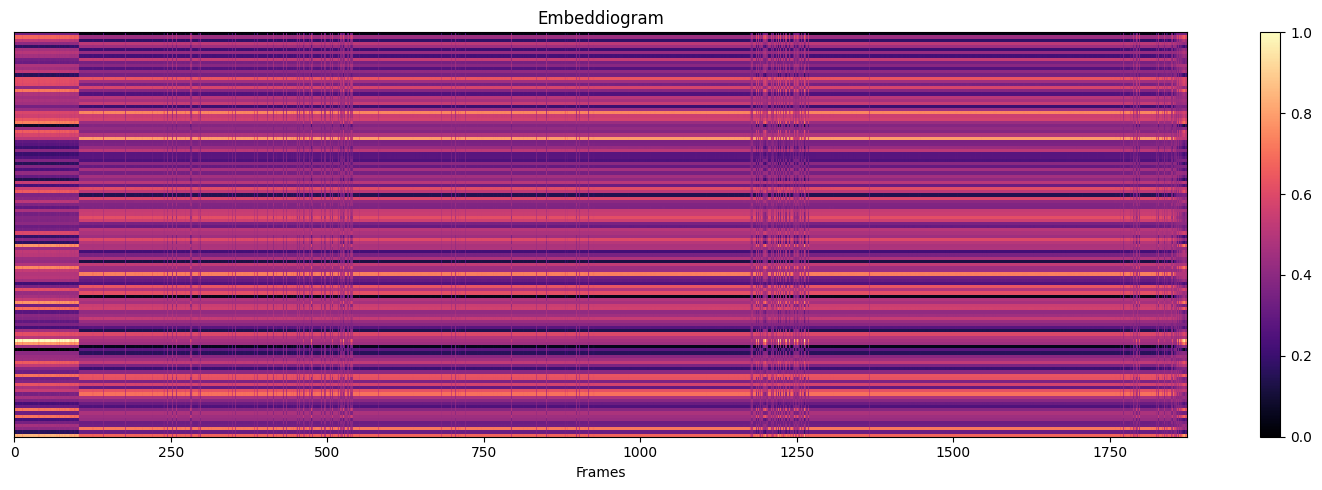
\includegraphics[width=\textwidth]{figures/images/embeddiogram_SALAMI_track_2.png}
    \caption[Embeddiogram]{Caption}
    \label{fig:embeddiogram}
\end{figure}
